\documentclass[]{article}
\usepackage{lmodern}
\usepackage{amssymb,amsmath}
\usepackage{ifxetex,ifluatex}
\usepackage{fixltx2e} % provides \textsubscript
\ifnum 0\ifxetex 1\fi\ifluatex 1\fi=0 % if pdftex
  \usepackage[T1]{fontenc}
  \usepackage[utf8]{inputenc}
\else % if luatex or xelatex
  \ifxetex
    \usepackage{mathspec}
  \else
    \usepackage{fontspec}
  \fi
  \defaultfontfeatures{Ligatures=TeX,Scale=MatchLowercase}
\fi
% use upquote if available, for straight quotes in verbatim environments
\IfFileExists{upquote.sty}{\usepackage{upquote}}{}
% use microtype if available
\IfFileExists{microtype.sty}{%
\usepackage{microtype}
\UseMicrotypeSet[protrusion]{basicmath} % disable protrusion for tt fonts
}{}
\usepackage[margin=1in]{geometry}
\usepackage{hyperref}
\hypersetup{unicode=true,
            pdfborder={0 0 0},
            breaklinks=true}
\urlstyle{same}  % don't use monospace font for urls
\usepackage{color}
\usepackage{fancyvrb}
\newcommand{\VerbBar}{|}
\newcommand{\VERB}{\Verb[commandchars=\\\{\}]}
\DefineVerbatimEnvironment{Highlighting}{Verbatim}{commandchars=\\\{\}}
% Add ',fontsize=\small' for more characters per line
\usepackage{framed}
\definecolor{shadecolor}{RGB}{248,248,248}
\newenvironment{Shaded}{\begin{snugshade}}{\end{snugshade}}
\newcommand{\AlertTok}[1]{\textcolor[rgb]{0.94,0.16,0.16}{#1}}
\newcommand{\AnnotationTok}[1]{\textcolor[rgb]{0.56,0.35,0.01}{\textbf{\textit{#1}}}}
\newcommand{\AttributeTok}[1]{\textcolor[rgb]{0.77,0.63,0.00}{#1}}
\newcommand{\BaseNTok}[1]{\textcolor[rgb]{0.00,0.00,0.81}{#1}}
\newcommand{\BuiltInTok}[1]{#1}
\newcommand{\CharTok}[1]{\textcolor[rgb]{0.31,0.60,0.02}{#1}}
\newcommand{\CommentTok}[1]{\textcolor[rgb]{0.56,0.35,0.01}{\textit{#1}}}
\newcommand{\CommentVarTok}[1]{\textcolor[rgb]{0.56,0.35,0.01}{\textbf{\textit{#1}}}}
\newcommand{\ConstantTok}[1]{\textcolor[rgb]{0.00,0.00,0.00}{#1}}
\newcommand{\ControlFlowTok}[1]{\textcolor[rgb]{0.13,0.29,0.53}{\textbf{#1}}}
\newcommand{\DataTypeTok}[1]{\textcolor[rgb]{0.13,0.29,0.53}{#1}}
\newcommand{\DecValTok}[1]{\textcolor[rgb]{0.00,0.00,0.81}{#1}}
\newcommand{\DocumentationTok}[1]{\textcolor[rgb]{0.56,0.35,0.01}{\textbf{\textit{#1}}}}
\newcommand{\ErrorTok}[1]{\textcolor[rgb]{0.64,0.00,0.00}{\textbf{#1}}}
\newcommand{\ExtensionTok}[1]{#1}
\newcommand{\FloatTok}[1]{\textcolor[rgb]{0.00,0.00,0.81}{#1}}
\newcommand{\FunctionTok}[1]{\textcolor[rgb]{0.00,0.00,0.00}{#1}}
\newcommand{\ImportTok}[1]{#1}
\newcommand{\InformationTok}[1]{\textcolor[rgb]{0.56,0.35,0.01}{\textbf{\textit{#1}}}}
\newcommand{\KeywordTok}[1]{\textcolor[rgb]{0.13,0.29,0.53}{\textbf{#1}}}
\newcommand{\NormalTok}[1]{#1}
\newcommand{\OperatorTok}[1]{\textcolor[rgb]{0.81,0.36,0.00}{\textbf{#1}}}
\newcommand{\OtherTok}[1]{\textcolor[rgb]{0.56,0.35,0.01}{#1}}
\newcommand{\PreprocessorTok}[1]{\textcolor[rgb]{0.56,0.35,0.01}{\textit{#1}}}
\newcommand{\RegionMarkerTok}[1]{#1}
\newcommand{\SpecialCharTok}[1]{\textcolor[rgb]{0.00,0.00,0.00}{#1}}
\newcommand{\SpecialStringTok}[1]{\textcolor[rgb]{0.31,0.60,0.02}{#1}}
\newcommand{\StringTok}[1]{\textcolor[rgb]{0.31,0.60,0.02}{#1}}
\newcommand{\VariableTok}[1]{\textcolor[rgb]{0.00,0.00,0.00}{#1}}
\newcommand{\VerbatimStringTok}[1]{\textcolor[rgb]{0.31,0.60,0.02}{#1}}
\newcommand{\WarningTok}[1]{\textcolor[rgb]{0.56,0.35,0.01}{\textbf{\textit{#1}}}}
\usepackage{graphicx,grffile}
\makeatletter
\def\maxwidth{\ifdim\Gin@nat@width>\linewidth\linewidth\else\Gin@nat@width\fi}
\def\maxheight{\ifdim\Gin@nat@height>\textheight\textheight\else\Gin@nat@height\fi}
\makeatother
% Scale images if necessary, so that they will not overflow the page
% margins by default, and it is still possible to overwrite the defaults
% using explicit options in \includegraphics[width, height, ...]{}
\setkeys{Gin}{width=\maxwidth,height=\maxheight,keepaspectratio}
\IfFileExists{parskip.sty}{%
\usepackage{parskip}
}{% else
\setlength{\parindent}{0pt}
\setlength{\parskip}{6pt plus 2pt minus 1pt}
}
\setlength{\emergencystretch}{3em}  % prevent overfull lines
\providecommand{\tightlist}{%
  \setlength{\itemsep}{0pt}\setlength{\parskip}{0pt}}
\setcounter{secnumdepth}{0}
% Redefines (sub)paragraphs to behave more like sections
\ifx\paragraph\undefined\else
\let\oldparagraph\paragraph
\renewcommand{\paragraph}[1]{\oldparagraph{#1}\mbox{}}
\fi
\ifx\subparagraph\undefined\else
\let\oldsubparagraph\subparagraph
\renewcommand{\subparagraph}[1]{\oldsubparagraph{#1}\mbox{}}
\fi

%%% Use protect on footnotes to avoid problems with footnotes in titles
\let\rmarkdownfootnote\footnote%
\def\footnote{\protect\rmarkdownfootnote}

%%% Change title format to be more compact
\usepackage{titling}

% Create subtitle command for use in maketitle
\providecommand{\subtitle}[1]{
  \posttitle{
    \begin{center}\large#1\end{center}
    }
}

\setlength{\droptitle}{-2em}

  \title{}
    \pretitle{\vspace{\droptitle}}
  \posttitle{}
    \author{}
    \preauthor{}\postauthor{}
    \date{}
    \predate{}\postdate{}
  

\begin{document}

\hypertarget{data-visualization-with-ggplot2}{%
\section{Data Visualization with
ggplot2}\label{data-visualization-with-ggplot2}}

Visualizing data is an area where R really shines. There are many ways
to plot data with R and these include base R,
\texttt{lattice},\texttt{grid} and , \texttt{ggplot2}. The only one we
will work with is \texttt{ggplot2}, which is now (I have no data to back
this up), the de-facto standard for visualizing data in R. Given that
\texttt{ggplot2} is general package for creating essentially ALL types
of visualizations, it can seem quite complex (and it is). What I hope
you will get out of this section is a basic understanding of how to
create a figure and, most importantly, how to find help and examples
that you can build off of for your own visualizations. If you want to
read more about why some people choose base plotting vs
\texttt{ggplot2}, the twitter/blogosphere ``argument'' between
\href{https://simplystatistics.org/2016/02/11/why-i-dont-use-ggplot2/}{Jeff
Leek} and \href{http://varianceexplained.org/r/why-I-use-ggplot2/}{David
Robinson} is worth some time.

\hypertarget{lesson-outline}{%
\subsection{Lesson Outline}\label{lesson-outline}}

\begin{itemize}
\tightlist
\item
  \protect\hyperlink{examples-of-greatness}{Examples of greatness}
\item
  \protect\hyperlink{basics-of-ggplot2}{Basics of \texttt{ggplot2}}
\item
  \protect\hyperlink{example-explained}{Example explained}
\end{itemize}

\hypertarget{exercise}{%
\subsection{Exercise}\label{exercise}}

\begin{itemize}
\tightlist
\item
  \protect\hyperlink{exercise-41}{Exercise 4.1}
\end{itemize}

\hypertarget{examples-of-what-is-possible}{%
\subsection{Examples of what is
possible}\label{examples-of-what-is-possible}}

Before we get started, I do like to show what is possible. A couple of
geospatial examples of maps created in R.

A few examples of maps built with R show this:

\begin{figure}
\centering
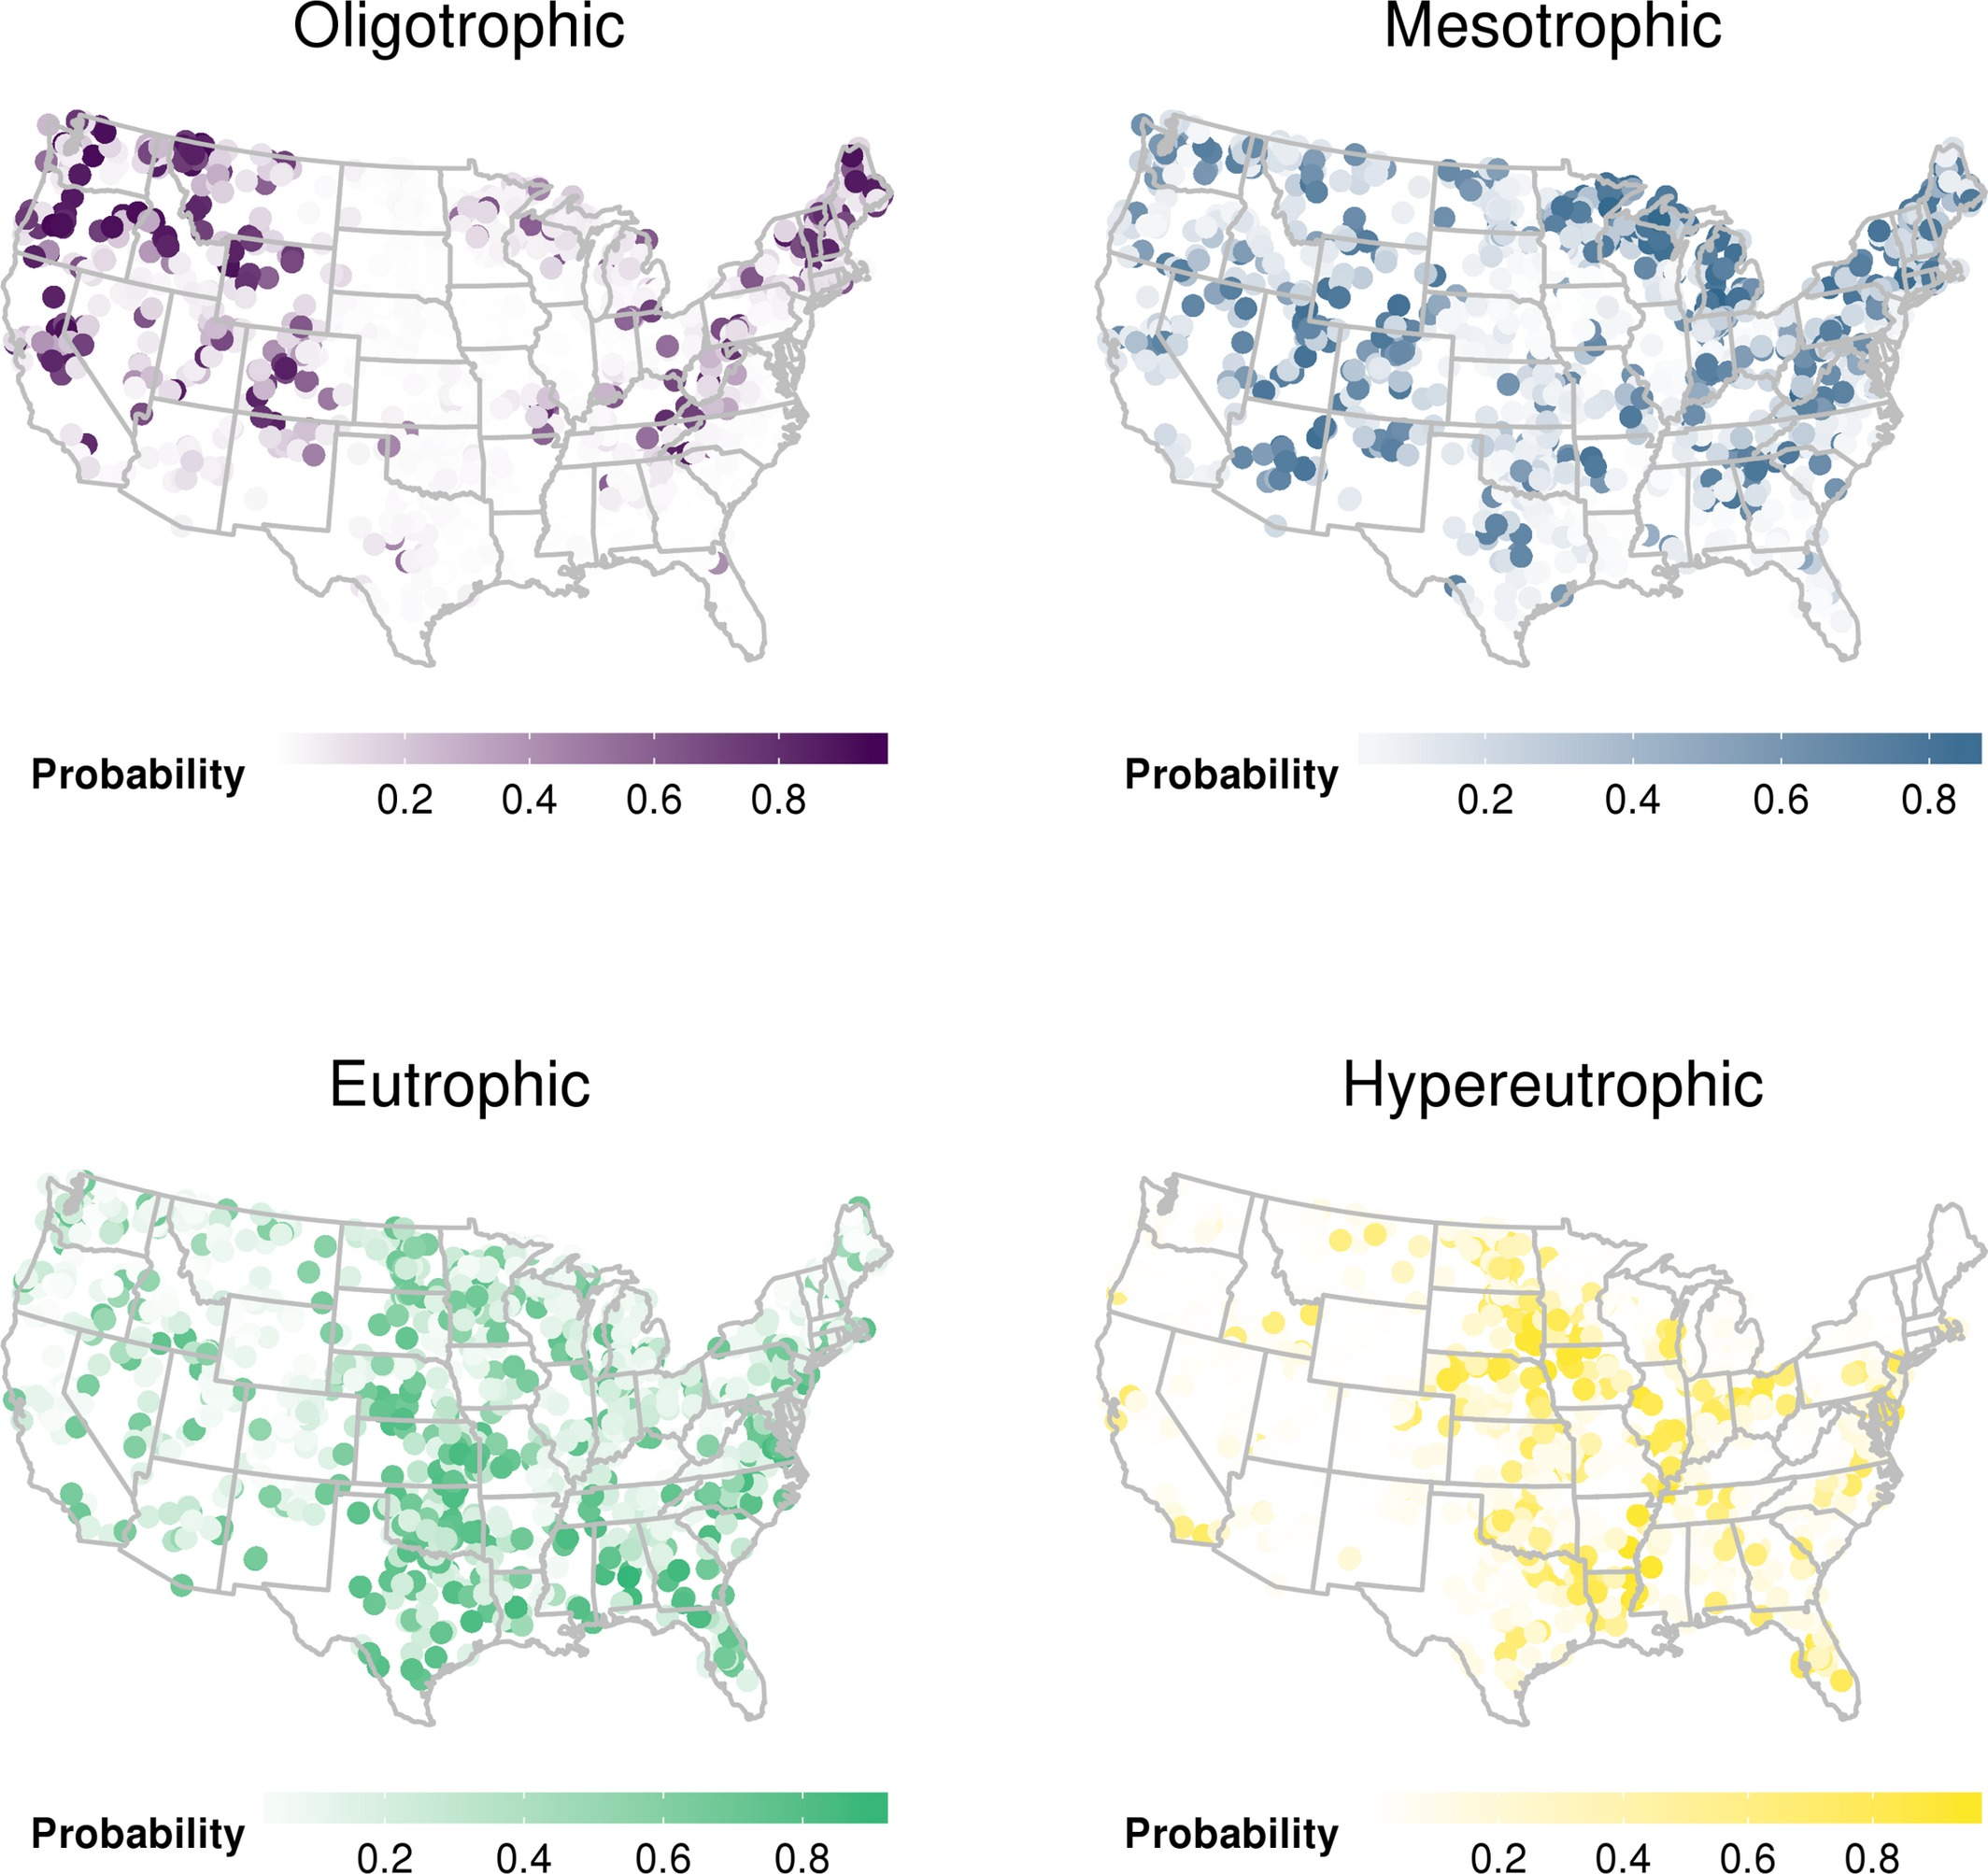
\includegraphics{figures/ecs21321-fig-0011-m.jpg}
\caption{Trophic State Modeling Results}
\end{figure}

\begin{figure}
\centering
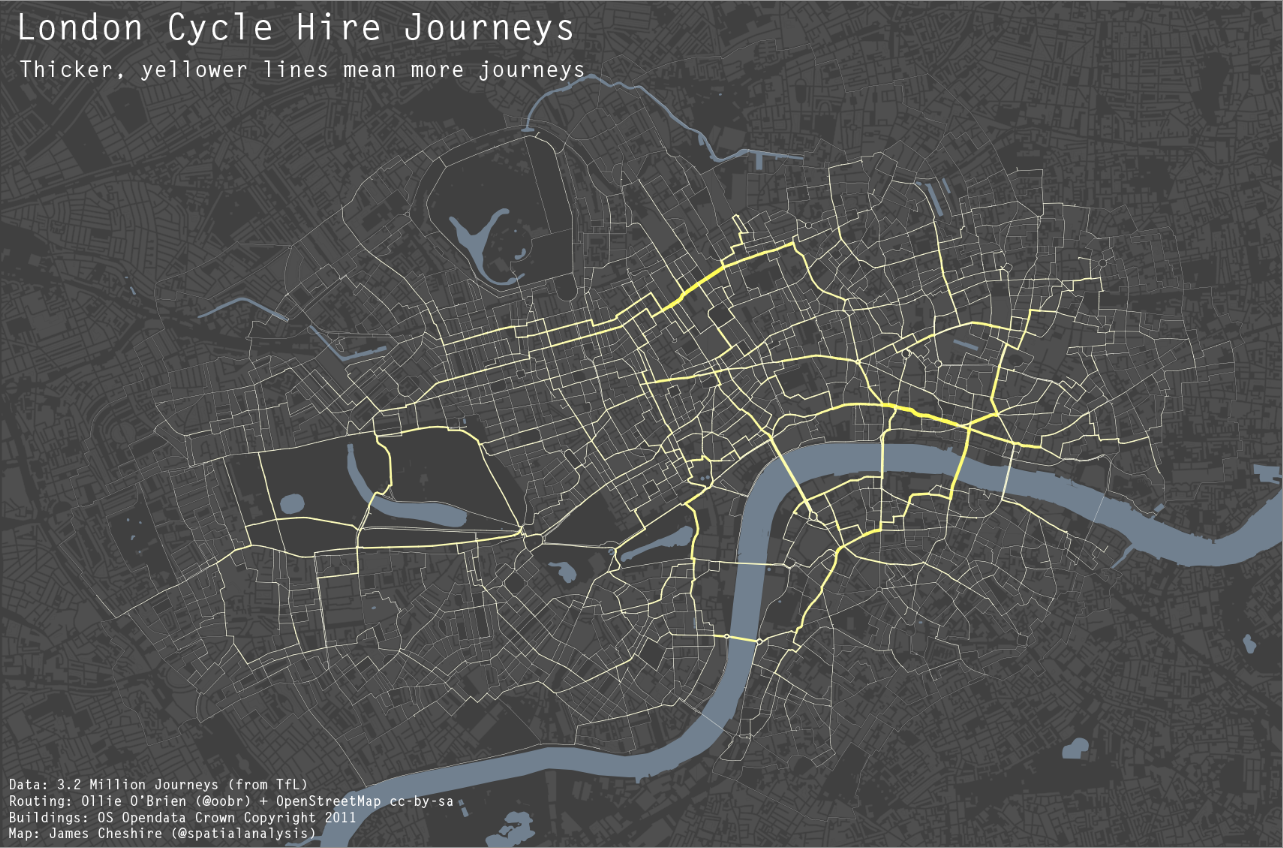
\includegraphics{figures/bike_ggplot.png}
\caption{London Bike Hires}
\end{figure}

\begin{figure}
\centering
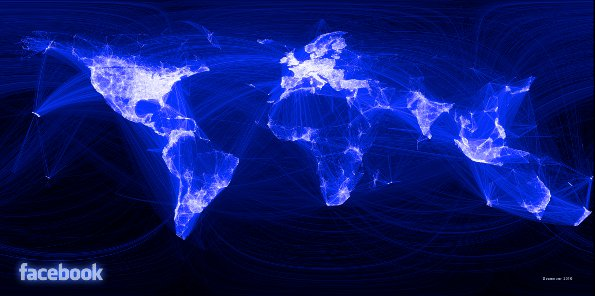
\includegraphics{figures/FbMap.jpg}
\caption{Facebook Users}
\end{figure}

More examples from Jeff's work

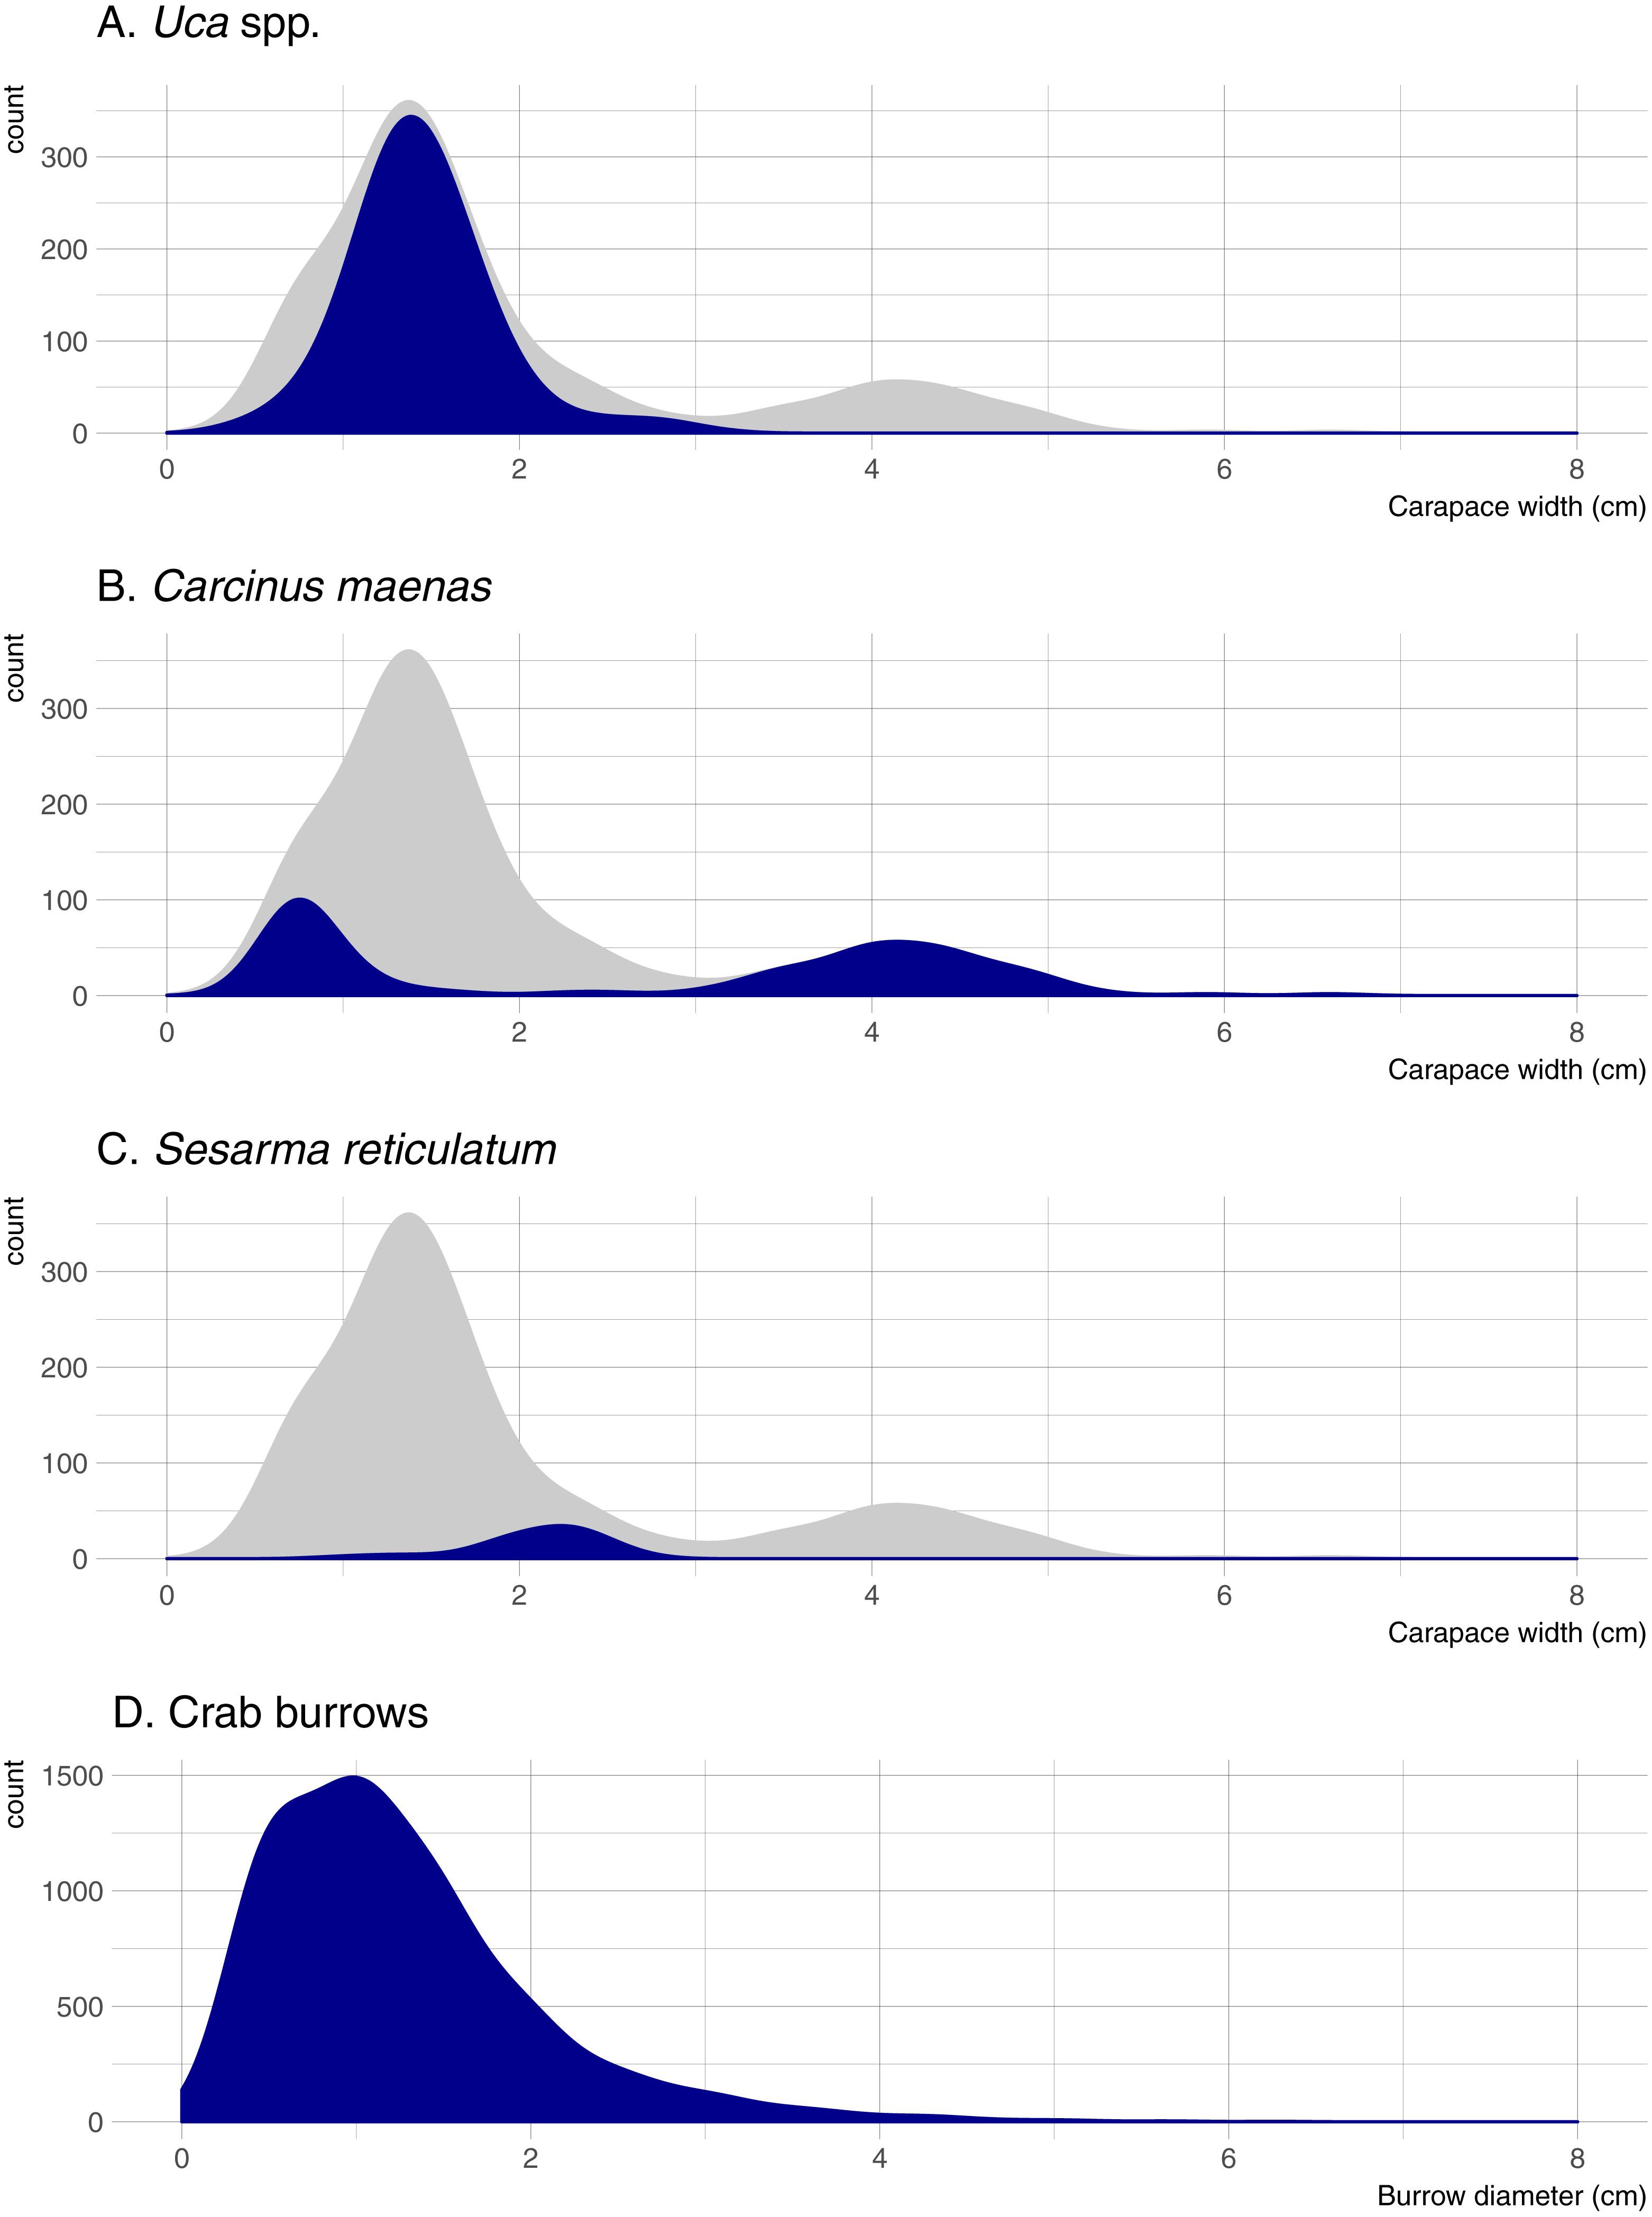
\includegraphics{figures/fig-2-full.png} from: Raposa et al.~(2018).
Top-down and bottom-up controls on overabundant New England salt marsh
crab populations. PeerJ. \url{https://doi.org/10.7717/peerj.4876}

\begin{figure}
\centering
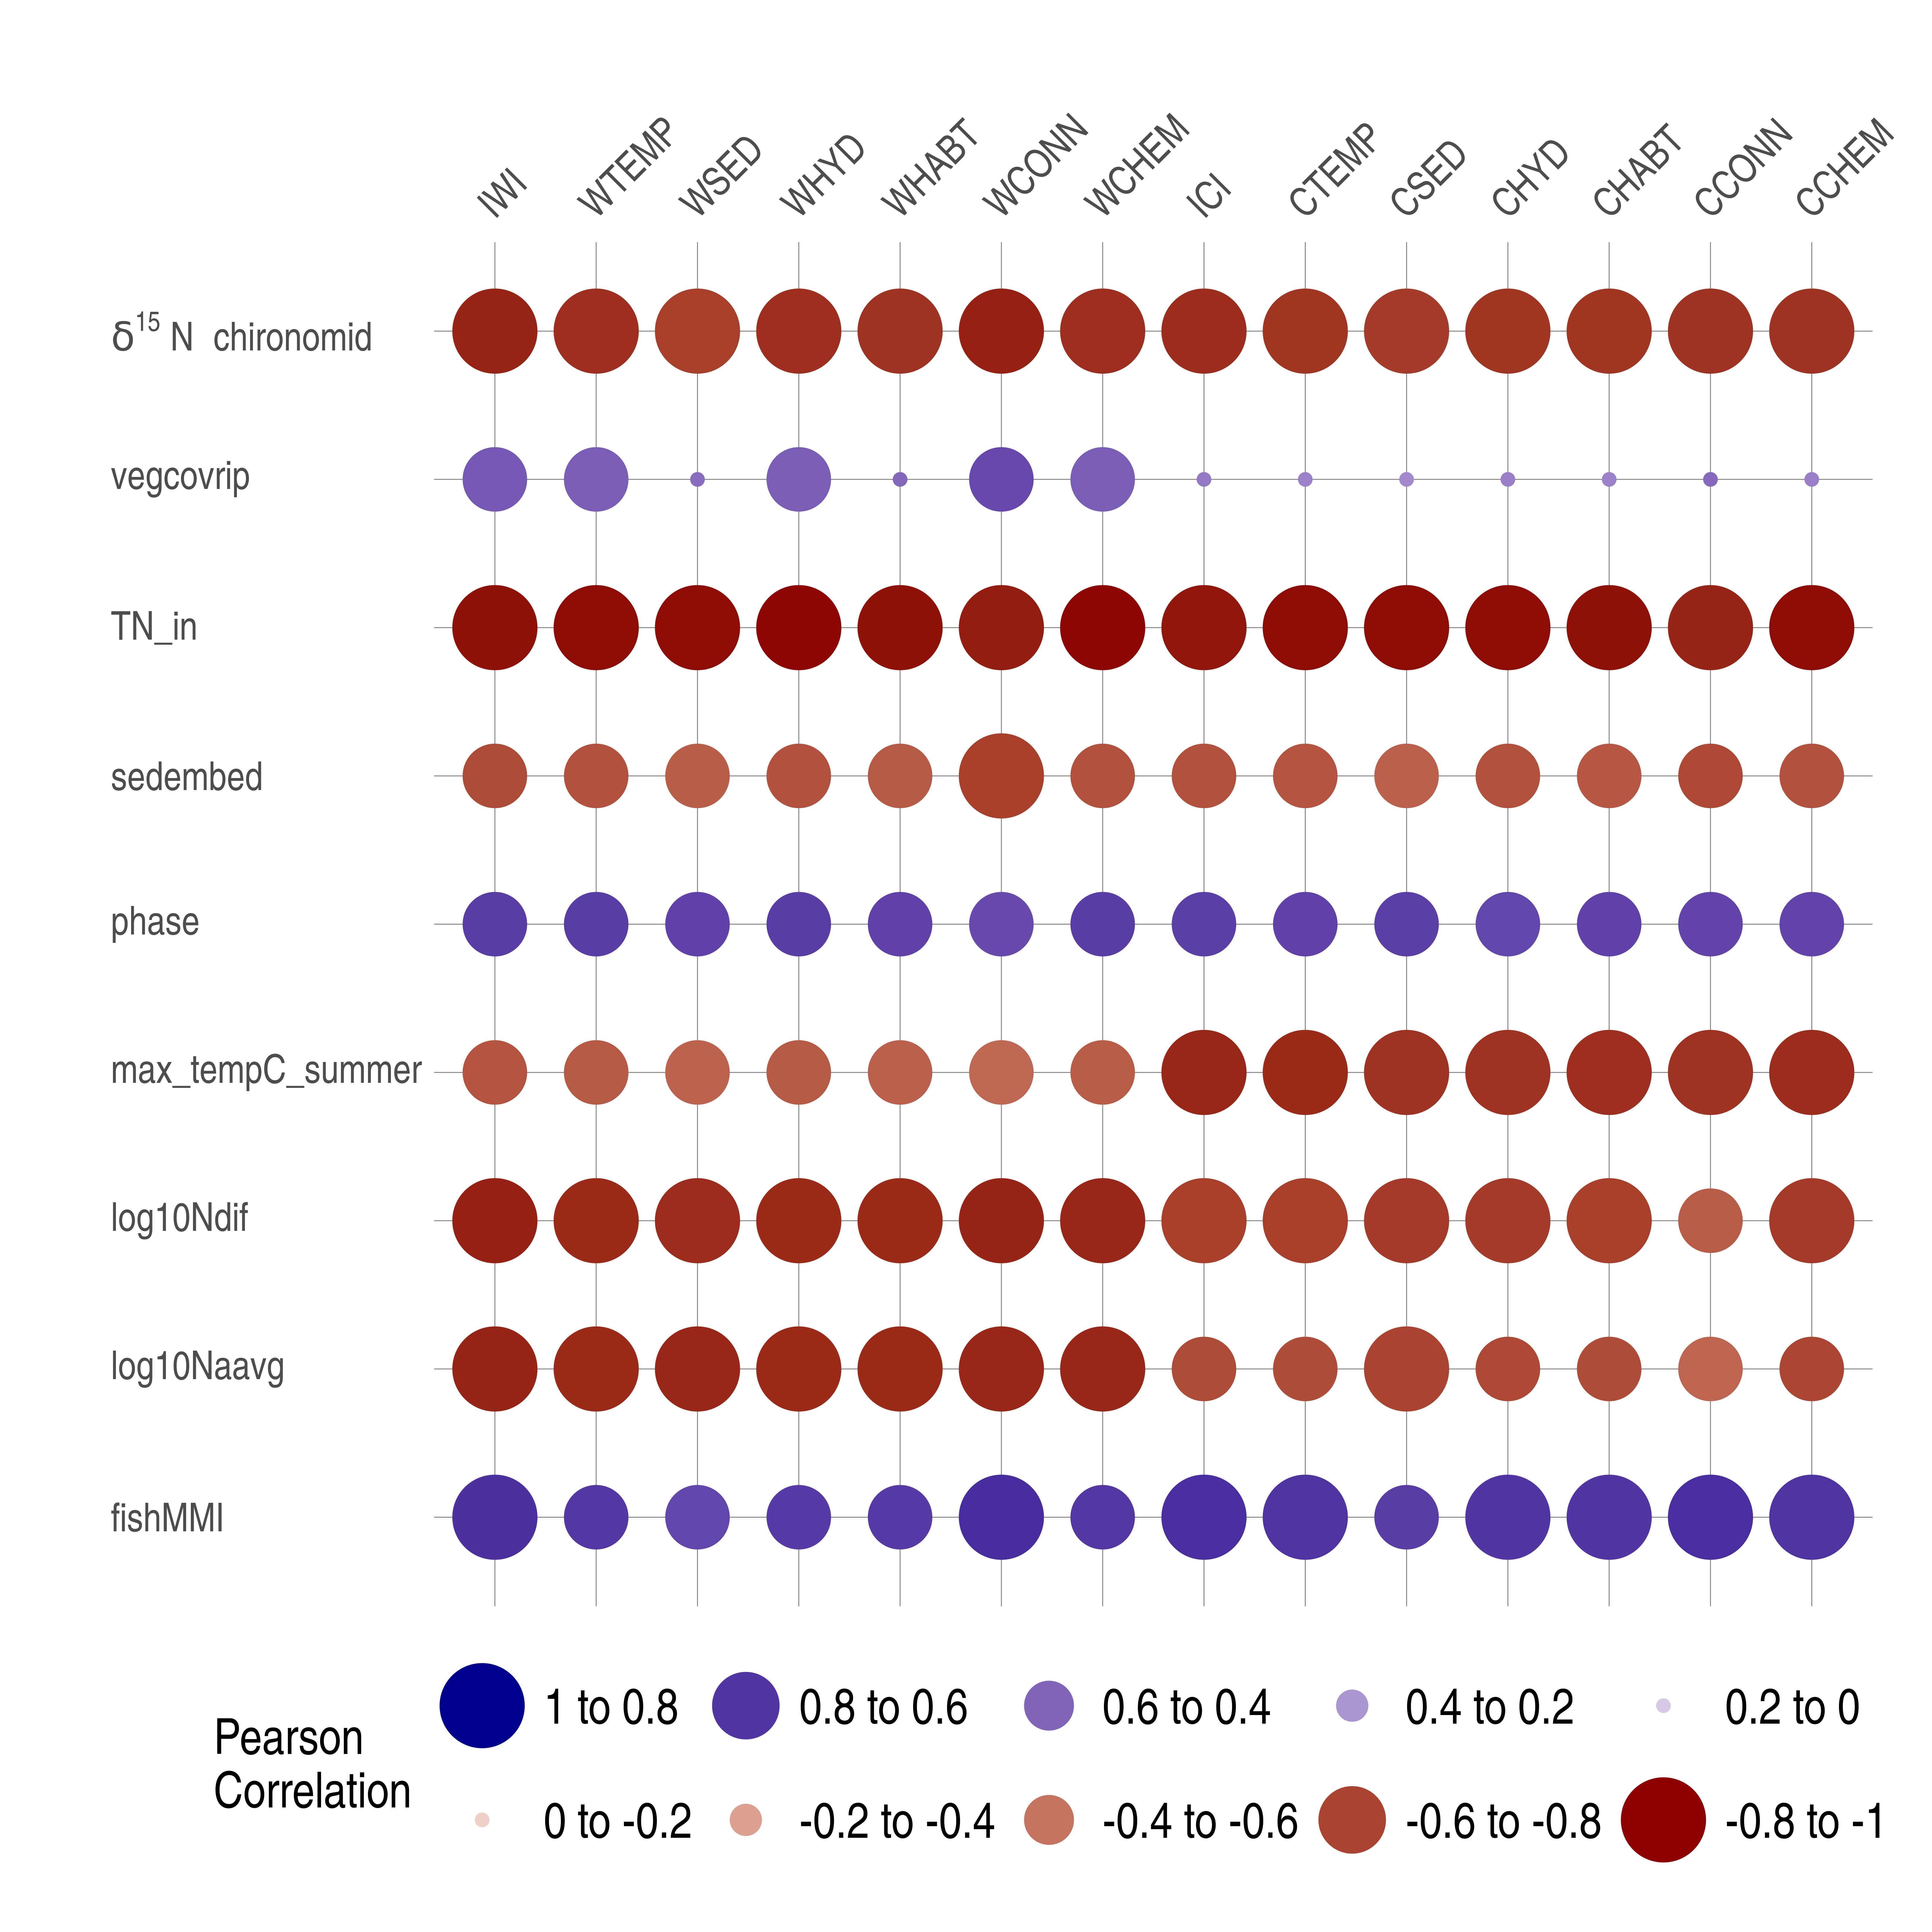
\includegraphics{figures/water-10-00604-g006.jpg}
\caption{heatmaps}
\end{figure}

from: Kuhn et al.~(2018) Performance of national maps of watershed
integrity at watershed scales. Water.
\url{https://doi.org/10.3390/w10050604}

And some cool examples using \texttt{ggplot2} with \texttt{plotly}.

\url{http://blog.revolutionanalytics.com/2014/11/3-d-plots-with-plotly.html}

Lastly, so that you know that there are many (often cool) mistakes that
lead up to a final visualization there is
\href{http://accidental-art.tumblr.com/}{Accidental aRt}. And for a
specific example \ldots{}

And the map I showed earlier of the trophic state probability had as one
of its early iterations this
\href{http://accidental-art.tumblr.com/post/96720455195/was-trying-to-mess-with-projections-in-ggplot}{``psychadelic
doughnut''}

\begin{figure}
\centering
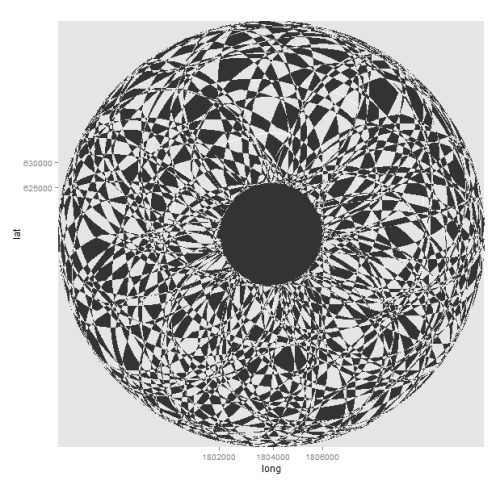
\includegraphics{figures/tumblr_nbfye5hrjR1smu039o1_500.jpg}
\caption{pd}
\end{figure}

(\textbf{ht to Anne Kuhn, my office mate, for the name})

A few other great links that I have recently found are also useful for
inspiration. First, is a repository on GitHub that has most (all?) of
the currently available color palletes in R:
\url{https://github.com/EmilHvitfeldt/r-color-palettes}. Second, the
\href{https://www.r-graph-gallery.com/}{R graph gallery} is a fantastic
resource for seeing all that is possible for visualization in R and the
code on how to do it!!

Now that we are sufficiently motivated, lets take a step back to the
very basics.

\hypertarget{introduction-to-ggplot2-scatterplot}{%
\subsection{\texorpdfstring{Introduction to \texttt{ggplot2}:
scatterplot}{Introduction to ggplot2: scatterplot}}\label{introduction-to-ggplot2-scatterplot}}

When you first get a dataset and are just starting to explore it, you
want do be able to quickly visualize different bits and pieces about the
data. I tend to do this, initially, with base R. But since our time is
short, we are going to focus our efforts just on \texttt{ggplot2}.

A lot has been written and discussed about \texttt{ggplot2}. In
particular see \href{http://ggplot2.org/}{here},
\href{http://docs.ggplot2.org/current/}{here} and
\href{https://github.com/karthikram/ggplot-lecture}{here}. The gist of
all this, is that \texttt{ggplot2} is an implementation of something
known as the ``grammar of graphics.'' This separates the basic
components of a graphic into distinct parts (e.g.~like the parts of
speech in a sentence). You add these parts together and get a figure.

Before we start developing some graphics, we need to do a bit of package
maintenance. If \texttt{ggplot2} had not be installed (it should be by
now), install it and make sure to load up the package with
\texttt{library()}

\begin{Shaded}
\begin{Highlighting}[]
\KeywordTok{install.packages}\NormalTok{(}\StringTok{"ggplot2"}\NormalTok{)}
\KeywordTok{library}\NormalTok{(}\StringTok{"ggplot2"}\NormalTok{)}
\end{Highlighting}
\end{Shaded}

With that finished, we can now use \texttt{ggplot2}. First thing we need
to do is to create our ggplot object. Everything will build off of this
object. The bare minimum for this is the data (handily,
\texttt{ggplot()} is expecting a data frame) and \texttt{aes()}, or the
aesthetics layers. Oddly (at least to me), this is the main place you
specify your x and y data values.

\begin{Shaded}
\begin{Highlighting}[]
\CommentTok{# aes() are the "aesthetics" mappings.  When you simply add the x and y}
\CommentTok{# that can seem a bit of a confusing term.  You also use aes() to }
\CommentTok{# change color, shape, size etc. of some items }
\NormalTok{iris_gg <-}\StringTok{ }\KeywordTok{ggplot}\NormalTok{(iris,}\KeywordTok{aes}\NormalTok{(}\DataTypeTok{x=}\NormalTok{Petal.Length,}\DataTypeTok{y=}\NormalTok{Petal.Width))}
\NormalTok{iris_gg}
\end{Highlighting}
\end{Shaded}

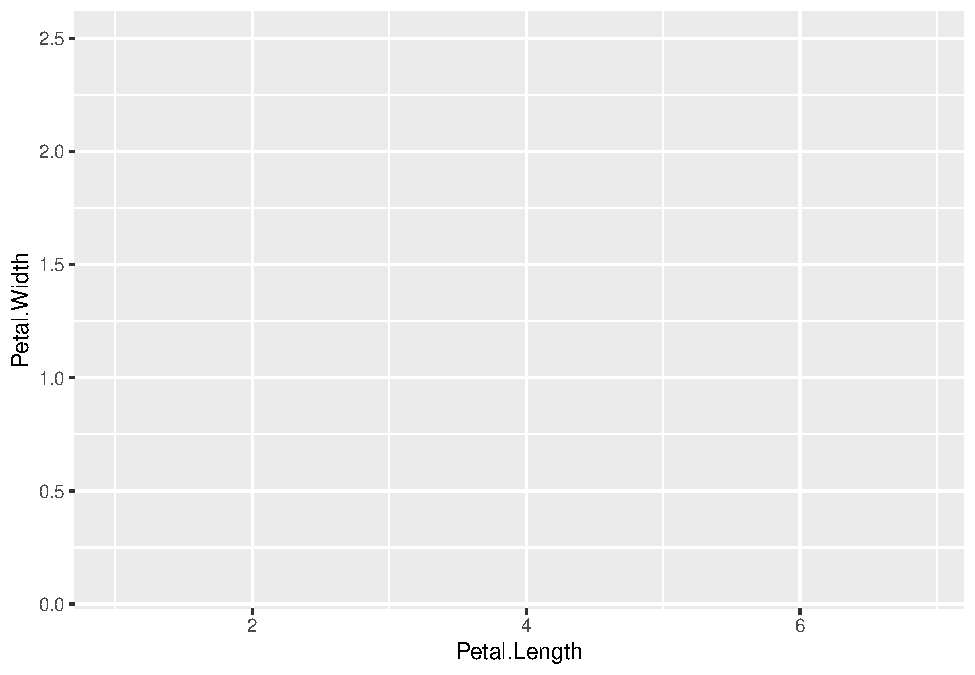
\includegraphics{figures/unnamed-chunk-2-1.pdf}

Great, nothing plotted\ldots{} All we did at this point is create an
object that contains our data and what we want on the x and y axes. We
haven't said anything about what type of plot we want to make. That
comes next with the use of geometries or \texttt{geom\_}'s.

So if we want to simply plot points we can add that geometry to the
ggplot object.

A side note on syntax. You will notice that we add new ``things'' to a
ggplot object by adding new functions. In concept this is somewhat
similar to the piping we talked about earlier. Essentially it takes the
output from the first function as the input to the second. So to add
points and create the plot, we would do:

\begin{Shaded}
\begin{Highlighting}[]
\CommentTok{#Different syntax than you are used to}
\NormalTok{iris_gg }\OperatorTok{+}\StringTok{ }
\StringTok{  }\KeywordTok{geom_point}\NormalTok{()}
\end{Highlighting}
\end{Shaded}

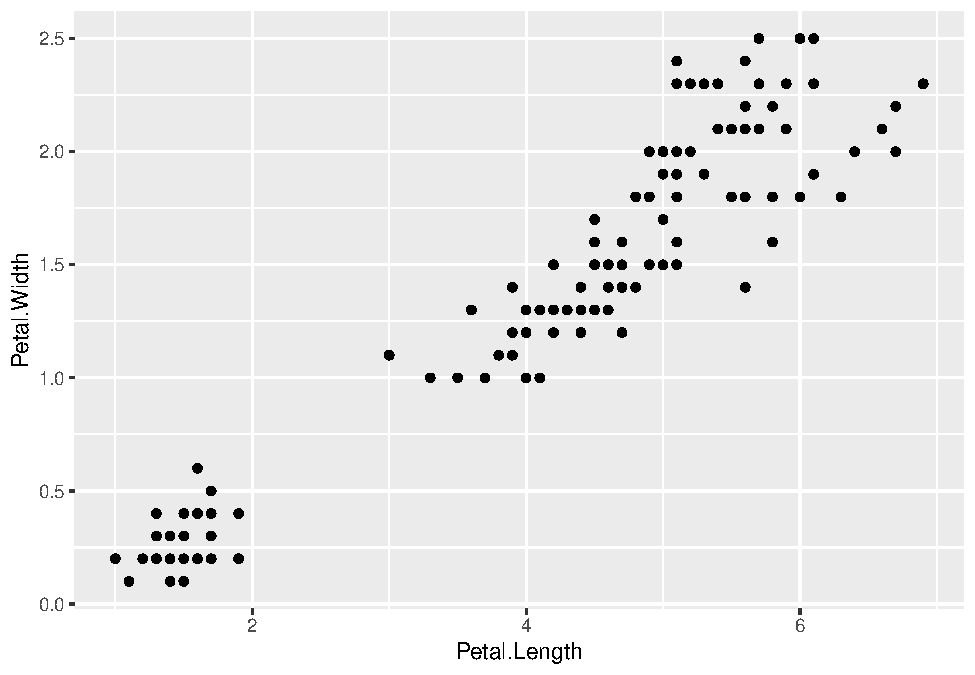
\includegraphics{figures/unnamed-chunk-3-1.pdf}

It is usually preferrable to save this to an object.

\begin{Shaded}
\begin{Highlighting}[]
\CommentTok{#This too can be saved to an object}
\NormalTok{iris_scatter <-}\StringTok{ }\NormalTok{iris_gg }\OperatorTok{+}
\StringTok{  }\KeywordTok{geom_point}\NormalTok{()}

\CommentTok{#Call it to show the plot}
\NormalTok{iris_scatter}
\end{Highlighting}
\end{Shaded}

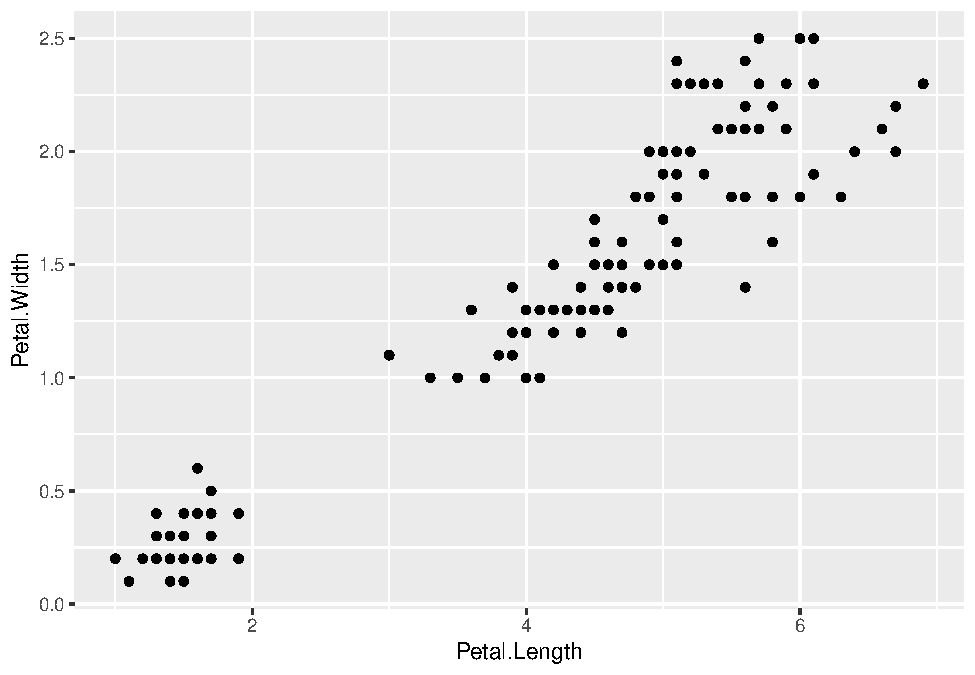
\includegraphics{figures/unnamed-chunk-4-1.pdf}

Not appreciably better than base, in my opinion. But what if we want to
add some stuff\ldots{}

First a title and some axis labels. These are part of \texttt{labs()}.

\begin{Shaded}
\begin{Highlighting}[]
\CommentTok{#Getting fancy to show italics and greek symbols}
\NormalTok{iris_scatter <-}\StringTok{ }\NormalTok{iris_scatter }\OperatorTok{+}
\StringTok{  }\KeywordTok{labs}\NormalTok{(}\DataTypeTok{title=}\StringTok{"Association Between Iris Petal measurements"}\NormalTok{,}
                     \DataTypeTok{x=}\StringTok{"Petal Length"}\NormalTok{, }\DataTypeTok{y=}\StringTok{"Petal Width"}\NormalTok{)}
\NormalTok{iris_scatter}
\end{Highlighting}
\end{Shaded}

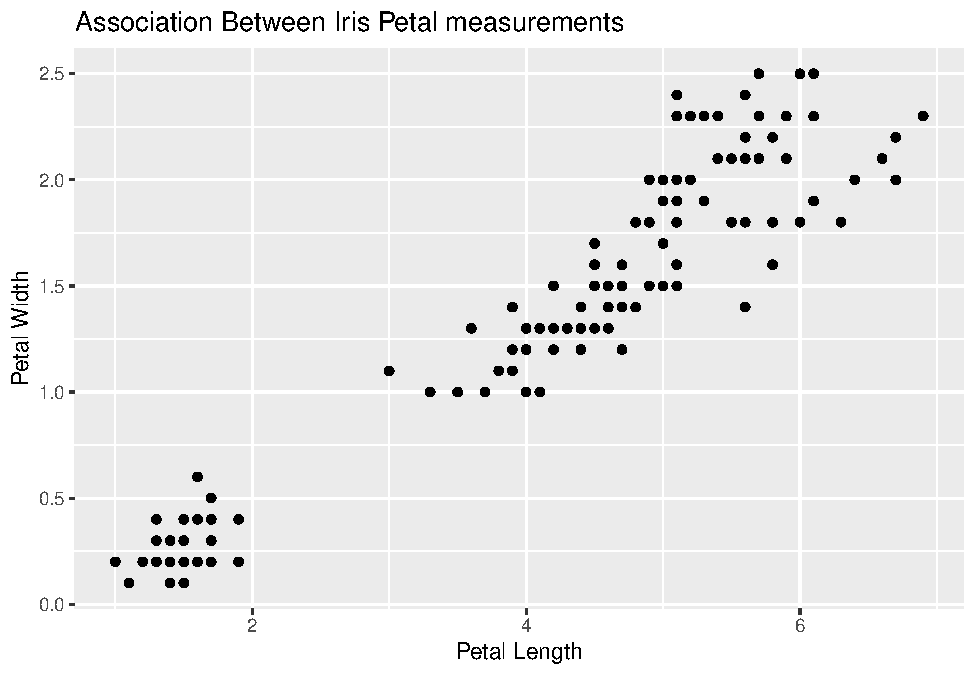
\includegraphics{figures/unnamed-chunk-5-1.pdf}

Now to add some colors, shapes etc to the point. Look at the
\texttt{geom\_point()} documentation for this.

\begin{Shaded}
\begin{Highlighting}[]
\NormalTok{iris_scatter <-}\StringTok{  }\NormalTok{iris_scatter }\OperatorTok{+}
\StringTok{  }\KeywordTok{geom_point}\NormalTok{(}\KeywordTok{aes}\NormalTok{(}\DataTypeTok{color=}\NormalTok{Species, }\DataTypeTok{shape=}\NormalTok{Species),}\DataTypeTok{size=}\DecValTok{2}\NormalTok{)}
\NormalTok{iris_scatter}
\end{Highlighting}
\end{Shaded}

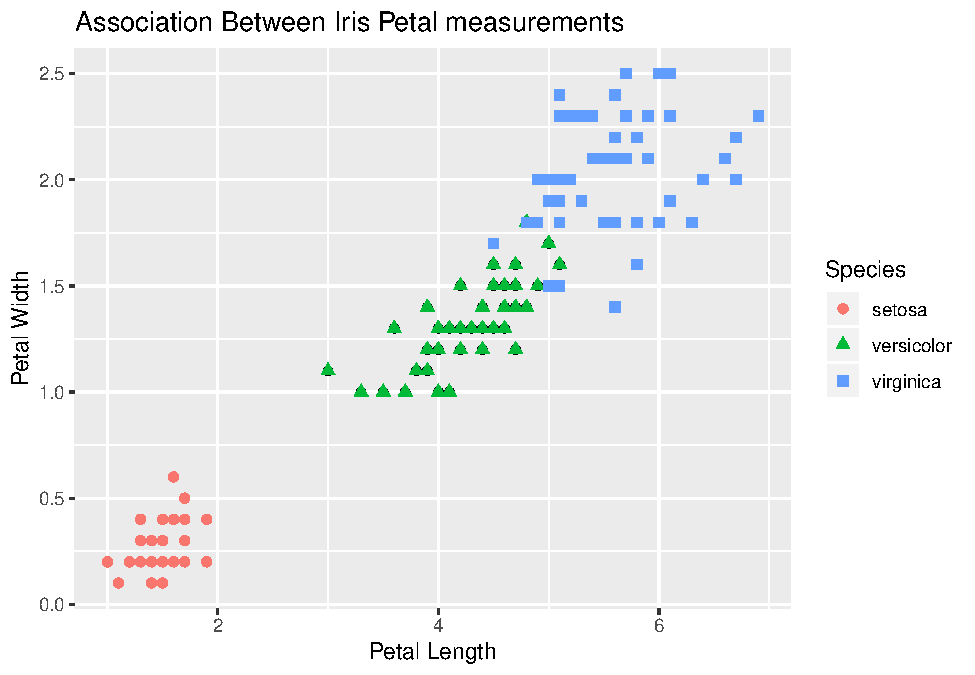
\includegraphics{figures/unnamed-chunk-6-1.pdf}

You'll notice we used \texttt{aes()} again, but this time inside of the
geometry. This tells ggplot2 that this aes only applies to the points.
Other geometries will not be affected by this.

In short, this is much easier than using base. Now \texttt{ggplot2}
really shines when you want to add stats (regression lines, intervals,
etc.).

Lets add a loess line with 95\% confidence intervals

\begin{Shaded}
\begin{Highlighting}[]
\NormalTok{iris_scatter_loess <-}\StringTok{ }\NormalTok{iris_scatter }\OperatorTok{+}
\StringTok{  }\KeywordTok{geom_smooth}\NormalTok{(}\DataTypeTok{method =} \StringTok{"loess"}\NormalTok{)}
\NormalTok{iris_scatter_loess}
\end{Highlighting}
\end{Shaded}

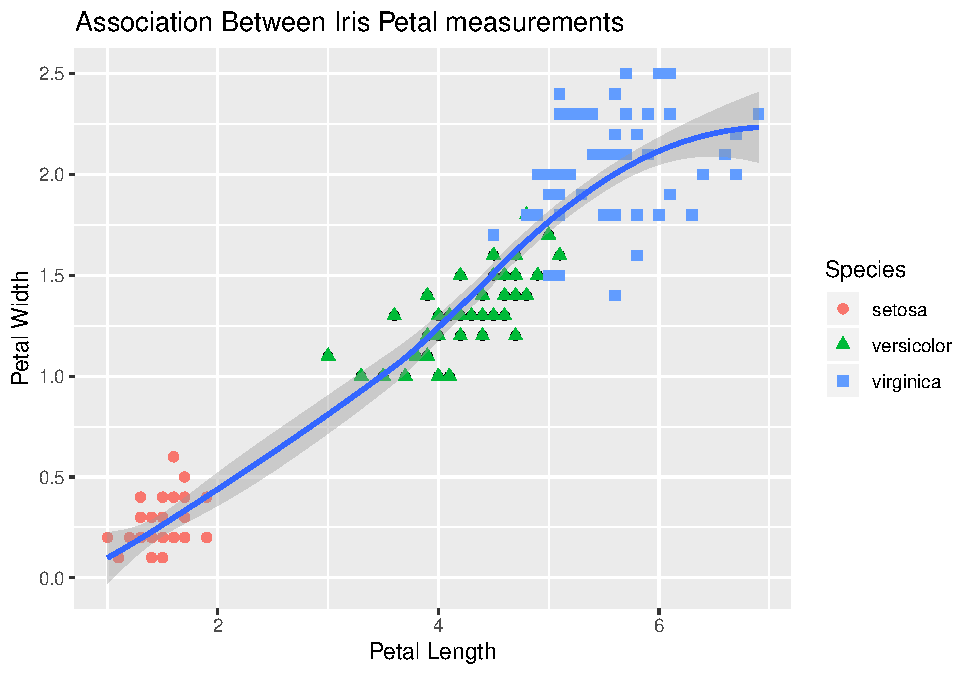
\includegraphics{figures/unnamed-chunk-7-1.pdf}

Try that in \texttt{base} with so little code!

Or we could add a linear regression line with:

\begin{Shaded}
\begin{Highlighting}[]
\NormalTok{iris_scatter_lm <-}\StringTok{ }\NormalTok{iris_scatter }\OperatorTok{+}
\StringTok{  }\KeywordTok{geom_smooth}\NormalTok{(}\DataTypeTok{method=}\StringTok{"lm"}\NormalTok{)}
\NormalTok{iris_scatter_lm}
\end{Highlighting}
\end{Shaded}

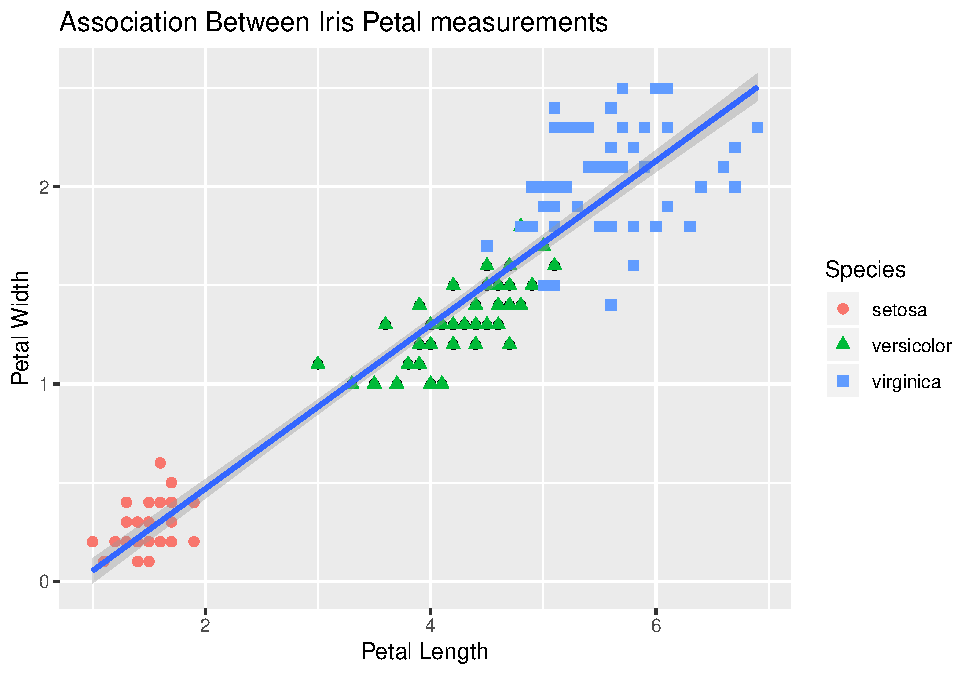
\includegraphics{figures/unnamed-chunk-8-1.pdf}

And if we are interested in the regressions by group we could do it this
way.

\begin{Shaded}
\begin{Highlighting}[]
\NormalTok{iris_scatter_lm_group <-}\StringTok{ }\NormalTok{iris_scatter }\OperatorTok{+}
\StringTok{  }\KeywordTok{geom_smooth}\NormalTok{(}\DataTypeTok{method=}\StringTok{"lm"}\NormalTok{, }\KeywordTok{aes}\NormalTok{(}\DataTypeTok{group=}\NormalTok{Species))}
\NormalTok{iris_scatter_lm_group}
\end{Highlighting}
\end{Shaded}

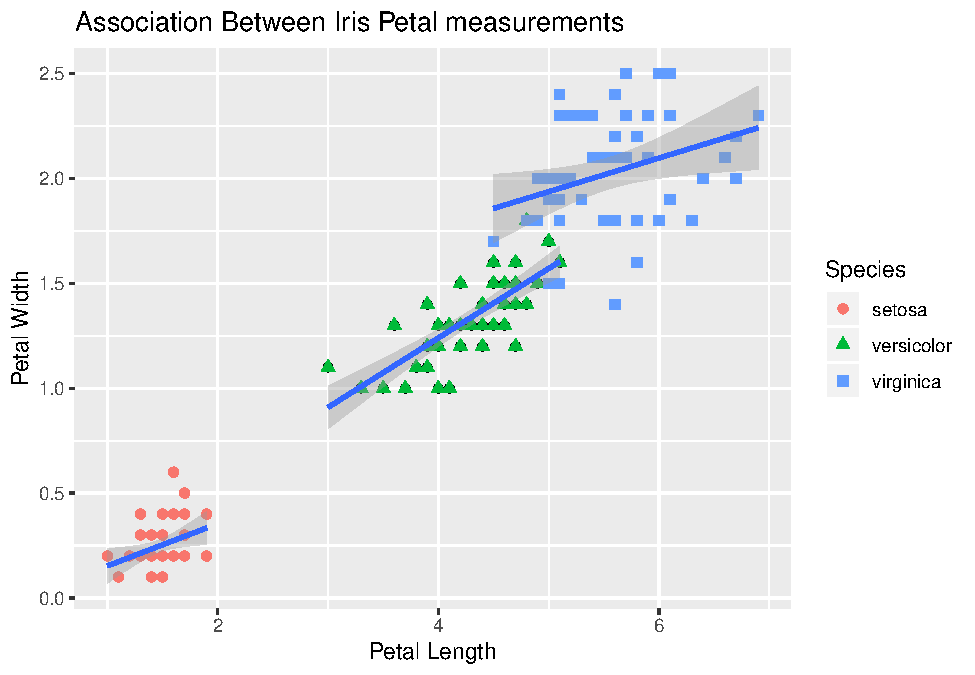
\includegraphics{figures/unnamed-chunk-9-1.pdf}

Or, if we wanted our regression lines to match the color.

\begin{Shaded}
\begin{Highlighting}[]
\NormalTok{iris_scatter_lm_color <-}\StringTok{ }\NormalTok{iris_scatter }\OperatorTok{+}\StringTok{ }
\StringTok{  }\KeywordTok{geom_smooth}\NormalTok{(}\DataTypeTok{method=}\StringTok{"lm"}\NormalTok{, }\KeywordTok{aes}\NormalTok{(}\DataTypeTok{color=}\NormalTok{Species))}
\NormalTok{iris_scatter_lm_color}
\end{Highlighting}
\end{Shaded}

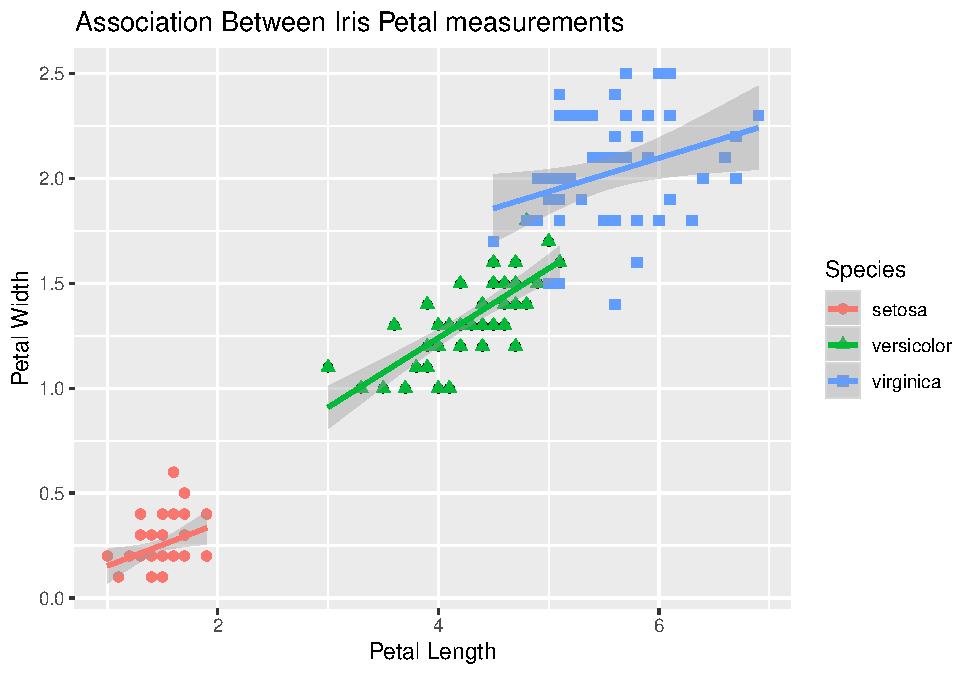
\includegraphics{figures/unnamed-chunk-10-1.pdf}

Notice, that we specified the \texttt{aes()} again, but for
\texttt{geom\_smooth()}. We only specified the x and y in the original
\texttt{ggplot} object, so if want to do something different in the
subsequent functions we need to overwrite it for the function in which
we want a different mapping (i.e.~groups).

In short, some of the initial setup for ggplot is a bit more verbose
than base R, but when we want to do some more complex plots it is much
easier in \texttt{ggplot2}.

Before we get into another exercise, lets look at some of the other
geometries. The best place to do this is excellent \texttt{ggplot2}
documentation of the \href{http://docs.ggplot2.org/current/}{geom
functions}.

\hypertarget{example-explained}{%
\subsection{Example explained}\label{example-explained}}

Now that we have the basics of \texttt{ggplot2} down, let's take a
closer look at our example in \texttt{nla\_analysis.R}.

\hypertarget{excercise-4.1}{%
\subsection{Excercise 4.1}\label{excercise-4.1}}

For this exercise we will work on creating a new plot from scratch. One
of the concepts I hope to get across is that creating a plot is as much
knowing data manipulation as it is knowing the details of your plotting
system (\texttt{ggplot2} in our case). Add some new code at the end of
our \texttt{nla\_anlaysis.R} that does the following

\begin{enumerate}
\def\labelenumi{\arabic{enumi}.}
\tightlist
\item
  Create a new data frame with the state by state average of total
  nitrogen, total phosphorus, and chlorophyll \emph{a}
\item
  Using this newly created data frame, plot mean total nitrogen on the
  x-axis, mean total phosphorus on the y-axis, and size and color the
  points based on the chlorophyll (extra credit if you log transform
  these data)
\item
  Try to use \texttt{ggplotly} from the \texttt{plotly} package to
  create an interactive version of this plot.
\item
  Don't forget to comment your code
\end{enumerate}

This will be a challenging excercise as it includes nearly all of the
tidyverse components we have talked about.


\end{document}
